% !TEX root = thesis.tex

\subsection{Hard processes}
\subsubsection{pQCD factorization}


%\begin{figure}[htb]
%\centering
%\includegraphics[width=0.5\textwidth]{pics/QCDLO}
%\caption[QCD Leading Order]{The basic pQCD processes and their quadratic matrix elements}
%\label{fig:qcdlo2}
%\end{figure}





The term Hard Scattering is used for the scattering of two point-like constituents (partons) of colliding nucleons, when the momentum transfer $Q^2$ is large ($Q \gg \Lambda_{\mathrm{QCD}}$). Figure ~\ref{fig:scattering} shows the incoming partons, quarks or gluons, as they exchange a space-like virtual gluon and produce two highly virtual outgoing partons. The outgoing partons will eventually fragment into collimated showers of partons, referred to as jets.

\begin{figure}[htb]
\centering
\documentclass{standalone}
\usepackage{tikz}
\usepackage{xcolor}
\usetikzlibrary{shapes,arrows}
\usetikzlibrary{trees}
\usetikzlibrary{shadows.blur}
\usetikzlibrary{positioning}
\usetikzlibrary{decorations.pathmorphing}
\usetikzlibrary{decorations.markings}
\begin{document}

\tikzset{
photon/.style={decorate, decoration={snake}, draw=red},
particlearrow/.style={draw=blue, postaction={decorate},
    decoration={markings,mark=at position .5 with {\arrow[draw=black]{>}}}},
antiparticlearrow/.style={draw=blue, postaction={decorate},
    decoration={markings,mark=at position .5 with {\arrow[draw=black]{>}}}},
particle/.style={draw=blue},
antiparticle/.style={draw=blue},
gluon/.style={decorate, draw=orange,
    decoration={coil,amplitude=4pt, segment length=5pt}}
 }
 
 
 
\tikzstyle{proton} = [ellipse, draw=black, text centered, fill=orange!20, minimum height=3em, blur shadow = {shadow blur steps=5},minimum width=1em ] 
\begin{tikzpicture}[node distance=1cm and 1.5cm]
\coordinate[] (p1);
\node[proton, right of=p1]  (proton)  {};
\coordinate[below right=-0.05cm and 0.02cm of proton] (aux1);
\coordinate[above right=-0.05cm and 0.02cm of proton] (aux2);
\coordinate[below right=0.0cm and 2cm of aux1] (vertex1);
\coordinate[right=2cm of aux2] (aux4);
\coordinate[right=2cm of proton] (aux5);
\coordinate[right=2cm of aux4] (spec1);
\coordinate[right=2cm of aux5] (spec2);

\coordinate[below right=1.5cm and 0.5cm of vertex1] (vertex2);

\coordinate[below right=0.0cm and 2cm of vertex2] (b1);
\node[proton, below right=-0.05cm and 0.02cm of b1] (proton2) {};
\coordinate[left=2cm of proton2] (aux6);
\coordinate[below left=-0.05cm and 0.02cm of proton2] (b2);
\coordinate[left=2cm of b2] (aux7);
\coordinate[left=2cm of aux7] (spec3);
\coordinate[left=2cm of aux6] (spec4);
\coordinate[right of=proton2] (p2);
\coordinate[above right=1cm and 1cm of vertex1] (jet1);
\coordinate[below left=1cm and 1cm of vertex2] (jet2);


%Jet cones
\coordinate[above right=1cm and 0.5cm of jet1] (cone11);
\coordinate[above right=0.5cm and 1cm of jet1, label={right:Jet}] (cone12);
\draw[particle] (jet1) -- (cone11);
\draw[particle] (jet1) -- (cone12);
\draw[blue] (cone11) to[out=45,in=45]  (cone12);
\draw[blue] (cone11) to[out=225,in=225] (cone12);

\coordinate[below left=1cm and 0.5cm of jet2] (cone21);
\coordinate[below left=0.5cm and 1cm of jet2, label={left:Jet}] (cone22);
\draw[particle] (jet2) -- (cone21);
\draw[particle] (jet2) -- (cone22);
\draw[blue] (cone21) to[out=45,in=45]  (cone22);
\draw[blue] (cone21) to[out=225,in=225] (cone22);

\draw[particlearrow] (p1) -- node[label=above:$P_A$] {} (proton); 
\draw[particlearrow] (aux1) -- node[label=below:$x_a$] {} (vertex1); 
\draw[particlearrow] (aux2) -- (aux4); 
\draw[particlearrow] (proton) -- (aux5);
\draw[particle] (aux4) -- (spec1);
\draw[particle] (aux5) -- (spec2);
\draw[particle] (aux7) -- (spec3);
\draw[particle] (aux6) -- (spec4);
\draw[particle] (vertex1) -- (jet1);
\draw[particle] (vertex2) -- (jet2);

\draw[gluon] (vertex1) -- node[label=right:$q$] {} (vertex2);
\draw[particlearrow] (b1) -- node[label=above:$x_b$] {} (vertex2);
\draw[particlearrow] (b2) -- (aux7);
\draw[particlearrow] (proton2) -- (aux6);

\draw[particlearrow] (p2) -- node[label=above:$P_B$] {} (proton2);




\end{tikzpicture}



\end{document}

%\includegraphics[width=0.5\textwidth]{pics/ink}
\caption[Hard scattering]{Schematic view of hard scattering process between two protons, producing two jets}
\label{fig:scattering}
\end{figure}

Historically one would study hard scatterings foremost with inclusive hadron spectra. In this context hadron production from hard scatterings can be factorised into three components; the parton distribution functions $f_a$, $f_b$ that give the probability of getting a parton with momentum fraction $x$ of the proton, the cross section of the elementary scattering $ab\rightarrow cd$,  and the fragmentation functions that give the probability of getting hadron $h$ from the parton.

\begin{equation}
\frac{\mathrm{d} \sigma^h_{pp}}{\mathrm{d}y\mathrm{d}^2\pt{}} = K \Sigma_{abcd}\int \mathrm{d}x_a \mathrm{d}x_b f_a\left(x_a,Q^2\right) f_b\left(x_b, Q^2\right) \frac{\mathrm{d} \sigma}{\mathrm{d}t}\left(ab\rightarrow cd \right)\frac{D_{h/c}^0}{\pi z_c},
\end{equation}

\noindent where 

\begin{equation}
x_{a,b} = \frac{\left| p_{a,b} \right|}{\left| p_{proton} \right|}.
\end{equation}


Parton distribution functions will be discussed further in the following section. The elementary cross section $ab\rightarrow cd$ can be calculated from QCD. A summary of the first order $2\rightarrow2$ processes in QCD is shown in Figure ~\ref{fig:qcdlo}. 

The final component in the factorization, fragmentation functions, describe the distribution of the fractional momenta of fragments radiated from the outgoing parton.  In a leading order picture, it can be interpreted as the probability that the observed final state originates from a given parton~\cite{Metz:2016swz}. Like the PDFs they are non-perturbative and must be determined experimentally. Most measurements come from $e^+ e^-$ collisions where the kinematics are better controlled. 


%
%\begin{figure}
%\centering
%\includegraphics[width=0.9\textwidth]{pics/Showering}
%\caption[Jet showering]{REPLACE FIGURE An illustration of jet showering. The highly virtual parton from the hard scattering will produce a shower of softer partons. When the virtuality is low enough the shower will go through a hadronisation process that produces the hadrons, which will be eventually observed in the detector. }
%\label{fig:highpt}
%\end{figure}



\begin{figure}[tb]
\centering
\documentclass{standalone}
\usepackage{tikz}
\usepackage{array}
\usetikzlibrary{shapes,arrows}
\usetikzlibrary{trees}
\usetikzlibrary{shadows.blur}
\usetikzlibrary{positioning}
\usetikzlibrary{decorations.pathmorphing}
\usetikzlibrary{decorations.markings}
\begin{document}
\newcommand{\centered}[1]{\begin{tabular}{l} #1 \end{tabular}}

\tikzset{
photon/.style={decorate, decoration={snake}, draw=red},
particlearrow/.style={draw=black, postaction={decorate},
    decoration={markings,mark=at position .5 with {\arrow[draw=black]{>}}}},
antiparticlearrow/.style={draw=black, postaction={decorate},
    decoration={markings,mark=at position .5 with {\arrow[draw=black]{>}}}},
particle/.style={draw=black},
antiparticle/.style={draw=blue},
gluon/.style={decorate, draw=black,
    decoration={coil,amplitude=2pt, segment length=3pt}}
 }
 
%\begin{tabular}{ >{\centering\arraybackslash} m{2cm} >{\centering\arraybackslash} m{2cm} >{\centering\arraybackslash} m{8cm}}
\begin{tabular}{ c c c}

\begin{tabular}{c}
$qq' \rightarrow qq' $ \\
$\bar q q' \rightarrow \bar qq' $
\end{tabular} 
& $\frac{4}{9}\frac{\hat s^2+\hat u^2}{\hat t^2}$

&
\centered{

 \begin{tikzpicture}[node distance=1cm and 1.5cm]
\coordinate[] (e1);
\coordinate[right=1cm of e1] (aux1);
\coordinate[right=1cm of aux1] (e2);
\coordinate[below=1cm of aux1] (aux2);
\coordinate[left=1cm of aux2] (e3);
\coordinate[right=1cm of aux2] (e4);

\draw[particle] (e1) -- (aux1);
\draw[particle] (aux1) -- (e2);
\draw[particle] (e3) -- (aux2);
\draw[particle] (aux2) -- (e4);
\draw[gluon] (aux2) -- node[label=left:$t$] {} (aux1);
\end{tikzpicture} 

}
 \\
$qq \rightarrow qq$ & $\frac{4}{9}\left( \frac{\hat s^2+\hat u^2}{\hat t^2} + \frac{\hat s^2+\hat u^2}{\hat t^2}  \right) - \frac{8}{27}\frac{\hat s^2}{\hat u \hat t}$ &
\centered{

\begin{tikzpicture}[node distance=1cm and 1.5cm]
\coordinate[] (e1);
\coordinate[right=1cm of e1] (aux1);
\coordinate[right=1cm of aux1] (e2);
\coordinate[below=1cm of aux1] (aux2);
\coordinate[left=1cm of aux2] (e3);
\coordinate[right=1cm of aux2] (e4);

\draw[particlearrow] (e1) -- (aux1);
\draw[particlearrow] (aux1) -- (e2);
\draw[particlearrow] (e3) -- (aux2);
\draw[particlearrow] (aux2) -- (e4);
\draw[gluon] (aux2) -- node[label=left:$t$] {} (aux1);
\end{tikzpicture} 

\begin{tikzpicture}[node distance=1cm and 1.5cm]
\coordinate[] (e1);
\coordinate[right=1cm of e1] (aux1);
\coordinate[right=1cm of aux1] (e2);
\coordinate[below=1cm of aux1] (aux2);
\coordinate[left=1cm of aux2] (e3);
\coordinate[right=1cm of aux2] (e4);

\draw[particlearrow] (e1) -- (aux1);
\draw[particle] (aux1) -- (e4);
\draw[particlearrow] (e3) -- (aux2);
\draw[particle] (aux2) -- (e2);
\draw[gluon] (aux2) -- node[label=left:$u$] {} (aux1);
\end{tikzpicture}
}
\\
$\bar q q \rightarrow \bar q' q'$ & $\frac{4}{9}\frac{\hat t^2+\hat u^2}{\hat s^2}$ &
\centered{
\begin{tikzpicture}[node distance=1cm and 1.5cm]
\coordinate[] (e1);
\coordinate[below right=0.7cm of e1] (aux1);
\coordinate[right=1cm of aux1] (aux2);
\coordinate[above right=0.7cm of aux2] (e2);
\coordinate[below left=0.7cm of aux1] (e3);
\coordinate[below right=0.7cm of aux2] (e4);

\draw[antiparticlearrow] (aux1) -- (e1);
\draw[antiparticlearrow] (e2) -- (aux2);
\draw[particlearrow] (e3) -- (aux1);
\draw[particlearrow] (aux2) -- (e4);
\draw[gluon] (aux2) -- node[label=above:$s$] {} (aux1);
\end{tikzpicture}
}
\\
$\bar q q \rightarrow \bar q q$ & $\frac{4}{9}\left( \frac{\hat s^2+\hat u^2}{\hat t^2} + \frac{\hat t^2+\hat u^2}{\hat s^2}  \right) - \frac{8}{27}\frac{\hat u^2}{\hat s \hat t}$ &
\centered{

\begin{tikzpicture}[node distance=1cm and 1.5cm]
\coordinate[] (e1);
\coordinate[below right=0.7cm of e1] (aux1);
\coordinate[right=1cm of aux1] (aux2);
\coordinate[above right=0.7cm of aux2] (e2);
\coordinate[below left=0.7cm of aux1] (e3);
\coordinate[below right=0.7cm of aux2] (e4);

\draw[antiparticlearrow] (aux1) -- (e1);
\draw[antiparticlearrow] (e2) -- (aux2);
\draw[particlearrow] (e3) -- (aux1);
\draw[particlearrow] (aux2) -- (e4);
\draw[gluon] (aux2) -- node[label=above:$s$] {} (aux1);
\end{tikzpicture}
\begin{tikzpicture}[node distance=1cm and 1.5cm]
\coordinate[] (e1);
\coordinate[right=1cm of e1] (aux1);
\coordinate[right=1cm of aux1] (e2);
\coordinate[below=1cm of aux1] (aux2);
\coordinate[left=1cm of aux2] (e3);
\coordinate[right=1cm of aux2] (e4);

\draw[antiparticlearrow] (e2) -- (aux1);
\draw[antiparticlearrow] (aux1) -- (e1);
\draw[particlearrow] (e3) -- (aux2);
\draw[particlearrow] (aux2) -- (e4);
\draw[gluon] (aux2) -- node[label=left:$t$] {} (aux1);
\end{tikzpicture} 
}
\\
$\bar q q \rightarrow gg$ & $\frac{32}{27}\frac{\hat u^2+\hat t^2}{\hat u \hat t} - \frac{8}{3}\frac{\hat u^2 + \hat t^2}{\hat s^2}$ &
\centered{

\begin{tikzpicture}
\coordinate[] (e1);
\coordinate[below right=0.7cm of e1] (aux1);
\coordinate[right=1cm of aux1] (aux2);
\coordinate[above right=0.7cm of aux2] (e2);
\coordinate[below left=0.7cm of aux1] (e3);
\coordinate[below right=0.7cm of aux2] (e4);

\draw[antiparticlearrow] (aux1) -- (e1);
\draw[gluon] (aux2) -- (e2);
\draw[particlearrow] (e3) -- (aux1);
\draw[gluon] (aux2) -- (e4);
\draw[gluon] (aux2) -- node[label=above:$s$] {} (aux1);
\end{tikzpicture}
}
\\
$gg \rightarrow \bar q q$ & $\frac{1}{6}\frac{\hat u^2+\hat t^2}{\hat u \hat t} - \frac{3}{8}\frac{\hat u^2 + \hat t^2}{\hat s^2}$ &
\centered{

\begin{tikzpicture}
\coordinate[] (e1);
\coordinate[below right=0.7cm of e1] (aux1);
\coordinate[right=1cm of aux1] (aux2);
\coordinate[above right=0.7cm of aux2] (e2);
\coordinate[below left=0.7cm of aux1] (e3);
\coordinate[below right=0.7cm of aux2] (e4);

\draw[gluon] (e1) -- (aux1);
\draw[antiparticlearrow] (e2) -- (aux2);
\draw[gluon] (e3) -- (aux1);
\draw[particlearrow] (aux2) -- (e4);
\draw[gluon] (aux2) -- node[label=above:$s$] {} (aux1);
\end{tikzpicture}
}
\\

$q g  \rightarrow qg $ & $\frac{4}{9}\frac{\hat u^2+\hat s^2}{\hat u \hat s} + \frac{\hat u^2 + \hat s^2}{\hat t^2}$ &
\centered{

\begin{tikzpicture}
\coordinate[] (e1);
\coordinate[below right=0.7cm of e1] (aux1);
\coordinate[right=1cm of aux1] (aux2);
\coordinate[above right=0.7cm of aux2] (e2);
\coordinate[below left=0.7cm of aux1] (e3);
\coordinate[below right=0.7cm of aux2] (e4);

\draw[gluon] (e1) -- (aux1);
\draw[gluon] (aux2) -- (e2);
\draw[particlearrow] (e3) -- (aux1);
\draw[particlearrow] (aux2) -- (e4);
\draw[particlearrow] (aux1) -- node[label=above:$s$] {} (aux2);
\end{tikzpicture}

\begin{tikzpicture}
\coordinate[] (e1);
\coordinate[below right=0.7cm of e1] (aux1);
\coordinate[right=1cm of aux1] (aux2);
\coordinate[above right=0.7cm of aux2] (e2);
\coordinate[below left=0.7cm of aux1] (e3);
\coordinate[below right=0.7cm of aux2] (e4);

\draw[gluon] (e1) -- (aux2);
\draw[gluon] (aux1) -- (e2);
\draw[particlearrow] (e3) -- (aux1);
\draw[particlearrow] (aux2) -- (e4);
\draw[particlearrow] (aux1) -- node[label=below:$s$] {} (aux2);
\end{tikzpicture}
\begin{tikzpicture}[node distance=1cm and 1.5cm]
\coordinate[] (e1);
\coordinate[right=1cm of e1] (aux1);
\coordinate[right=1cm of aux1] (e2);
\coordinate[below=1cm of aux1] (aux2);
\coordinate[left=1cm of aux2] (e3);
\coordinate[right=1cm of aux2] (e4);

\draw[gluon] (e1) -- (aux1);
\draw[gluon] (aux1) -- (e2);
\draw[particlearrow] (e3) -- (aux2);
\draw[particlearrow] (aux2) -- (e4);
\draw[gluon] (aux2) -- node[label=left:$t$] {} (aux1);
\end{tikzpicture} 
}
\\
$g g  \rightarrow gg $ & $\frac{9}{2}\left(3- \frac{\hat u \hat t}{\hat s^2}  - \frac{\hat u \hat s}{\hat t^2} -\frac{\hat s \hat t}{\hat u^2}\right)$ &
\centered{
\begin{tikzpicture}[node distance=1cm and 1.5cm]
\coordinate[] (e1);
\coordinate[right=1cm of e1] (aux1);
\coordinate[right=1cm of aux1] (e2);
\coordinate[below=1cm of aux1] (aux2);
\coordinate[left=1cm of aux2] (e3);
\coordinate[right=1cm of aux2] (e4);

\draw[gluon] (e1) -- (aux1);
\draw[gluon] (aux1) -- (e2);
\draw[gluon] (e3) -- (aux2);
\draw[gluon] (aux2) -- (e4);
\draw[gluon] (aux2) -- node[label=left:$t$] {} (aux1);
\end{tikzpicture} 
\begin{tikzpicture}
\coordinate[] (e1);
\coordinate[below right=0.7cm of e1] (aux1);
\coordinate[right=1cm of aux1] (aux2);
\coordinate[above right=0.7cm of aux2] (e2);
\coordinate[below left=0.7cm of aux1] (e3);
\coordinate[below right=0.7cm of aux2] (e4);

\draw[gluon] (e1) -- (aux1);
\draw[gluon] (aux2) -- (e2);
\draw[gluon] (e3) -- (aux1);
\draw[gluon] (aux2) -- (e4);
\draw[gluon] (aux2) -- node[label=above:$s$] {} (aux1);
\end{tikzpicture}

\begin{tikzpicture}[node distance=1cm and 1.5cm]
\coordinate[] (e1);
\coordinate[right=1cm of e1] (aux1);
\coordinate[right=1cm of aux1] (e2);
\coordinate[below=1cm of aux1] (aux2);
\coordinate[left=1cm of aux2] (e3);
\coordinate[right=1cm of aux2] (e4);

\draw[gluon] (e1) -- (aux1);
\draw[gluon] (aux1) -- (e4);
\draw[gluon] (e3) -- (aux2);
\draw[gluon] (aux2) -- (e2);
\draw[gluon] (aux2) -- node[label=left:$u$] {} (aux1);
\end{tikzpicture}

\begin{tikzpicture}
\coordinate[] (e1);
\coordinate[below right=0.7cm of e1] (aux1);
\coordinate[above right=0.7cm of aux1] (e2);
\coordinate[below left=0.7cm of aux1] (e3);
\coordinate[below right=0.7cm of aux1] (e4);

\draw[gluon] (e1) -- (aux1);
\draw[gluon] (aux1) -- (e2);
\draw[gluon] (e3) -- (aux1);
\draw[gluon] (aux1) -- (e4);
\end{tikzpicture}
}


\end{tabular}
\end{document}
\caption[QCD Leading Order]{The basic pQCD processes and their quadratic matrix elements}
\label{fig:qcdlo}
\end{figure}



\subsubsection*{Parton Distribution Function}
Parton Distribution Functions (PDFs) $f_a\left(x\right)$ give the differential probability for parton $a$ to carry momentum fraction $x$ of the proton momentum. %PDFs  are extracted from comprehensive global analysis of experimental results from a variety of fixed-target and collider experiments.
As the PDFs cannot be calculated from first principles they are measured in Deeply Inelastic Scattering (DIS) experiments~\cite{Placakyte:2011az} and are extrapolated to the relevant momentum scales using the Dokshitzer-Gribov-Lipatov-Altarelli-Parisi (DGLAP) evolution scheme ~\cite{Gribov:1972ri,Altarelli:1977zs,Dokshitzer:1977sg}  %~\ref{eq:dglap}.

\begin{equation}
\mu_\mathrm{F}^2 \frac{\partial f_i\left(x,\mu_{\mathrm{F}}^2 \right)}{\partial \mu_{\mathrm{F}}^2} = \Sigma_j \frac{\alpha_s\left(\mu_{\mathrm{F}}\right)}{2{pi}} \int _x^1 \frac{\mathrm{d}z}{z} P_{ij}(z) f_j\left(\frac{x}{z},\mu_{\mathrm{F}}^2\right),
\label{eq:dglap}
\end{equation}



\noindent where $\mu_{\mathrm{F}}$ is a factorization scale. The splitting functions $P_{ij}$ describe the probability to radiate parton $i$ with momentum fraction $z$ from parton $j$. Different theory interpretation and experimental data gives rise to different PDF's. Thus there are several commonly used PDF sets: CTEQ~\cite{cteq}, HERAPDF~\cite{CooperSarkar:2011aa}, PDF4LHC~\cite{Butterworth:2015oua}, etc. %Depending on the data used 

\subsubsection{Jet showering}
\label{sec:shower}
\begin{figure}
\centering
\documentclass{standalone}
\usepackage{tikz}
\usepackage{xcolor}
\usetikzlibrary{shapes,arrows}
\usetikzlibrary{trees}
\usetikzlibrary{shadows.blur}
\usetikzlibrary{positioning}
\usetikzlibrary{decorations.pathmorphing}
\usetikzlibrary{decorations.markings}
\begin{document}
\tikzset{
photon/.style={decorate, decoration={snake}, draw=red},
particlearrow/.style={draw=blue, line width=0.75pt, postaction={decorate},
    decoration={markings,mark=at position .5 with {\arrow[draw=black]{>}}}},
antiparticlearrow/.style={draw=blue, postaction={decorate},
    decoration={markings,mark=at position .5 with {\arrow[draw=black]{>}}}},
particle/.style={draw=blue, line width=0.75pt},
hadron/.style={draw=blue,line width=2pt,postaction={decorate},
    decoration={markings,mark=at position .9 with {\arrow[draw=blue]{>}}}},
antiparticle/.style={draw=blue},
gluon/.style={decorate, draw=orange, line width=0.75pt,
    decoration={coil,amplitude=4pt, segment length=5pt}}
 }
\begin{tikzpicture}
%\draw[step = 4cm, gray, thin] (-3cm,-3cm) grid(8,4cm);

\node[ellipse,draw=orange,fill=orange!20, minimum height=1cm, blur shadow = {shadow blur steps=5},minimum width=2cm] (hard) {};
\coordinate[above=1cm of hard, label=Hard Scattering] (label);
\coordinate[left=1cm of hard] (p1);
\coordinate[above left=1cm and 1cm of hard] (p2);
\coordinate[right=1cm of hard] (p3);
\coordinate[below right=1cm and 1cm of hard] (p4);

\coordinate[above right=1cm and 1.25cm of p3] (vertex1_1);
\coordinate[below right=1cm and 1.25cm of p3]  (vertex1_2);

\coordinate[above right=0.75cm and 1cm of vertex1_1] (vertex2_1);
\coordinate[below right=0.3cm and 1cm of vertex1_1] (vertex2_2);
\coordinate[above right=0.3cm and 1cm of vertex1_2] (vertex2_3);
\coordinate[below right=0.75cm and 1cm of vertex1_2] (vertex2_4);


\coordinate[above right=0.75cm and 1cm of vertex2_1] (vertex3_1);
\coordinate[below right=0.3cm and 1cm of vertex2_1] (vertex3_2);
\coordinate[above right=0.3cm and 1cm of vertex2_2] (vertex3_3);
\coordinate[below right=0.3cm and 1cm of vertex2_2] (vertex3_4);
\coordinate[above right=0.3cm and 1cm of vertex2_3] (vertex3_5);
\coordinate[below right=0.3cm and 1cm of vertex2_3] (vertex3_6);
\coordinate[above right=0.3cm and 1cm of vertex2_4] (vertex3_7);
\coordinate[below right=0.75cm and 1cm of vertex2_4] (vertex3_8);


\draw[particlearrow] (p1) -- (hard);
\draw[particlearrow] (p2) -- (hard);
\draw[particlearrow] (hard) -- (p3);
\draw[particlearrow] (hard) -- (p4);

\draw[particle] (p3) -- (vertex1_2);
\draw[gluon] (p3) -- (vertex1_1);

\draw[particle] (vertex1_1) -- (vertex2_1);
\draw[gluon] (vertex1_1) -- (vertex2_2);
\draw[gluon] (vertex1_2) -- (vertex2_3);
\draw[gluon] (vertex1_2) -- (vertex2_4);

\draw[gluon] (vertex2_1) -- (vertex3_1);
\draw[particle] (vertex2_1) -- (vertex3_2);
\draw[particle] (vertex2_2) -- (vertex3_3);
\draw[particle] (vertex2_2) -- (vertex3_4);
\draw[gluon] (vertex2_3) -- (vertex3_5);
\draw[gluon] (vertex2_3) -- (vertex3_6);
\draw[particle] (vertex2_4) -- (vertex3_7);
\draw[particle] (vertex2_4) -- (vertex3_8);

\node[rectangle,draw=orange, fill=orange!20, below right=-0.5cm and 0cm of vertex3_1,minimum width=1cm, minimum height=6cm,label={below:Hadronisation},blur shadow = {shadow blur steps=5}] (hadr) {};

\coordinate[right=0cm of hadr] (hadron1);
\coordinate[right=2cm of hadron1] (detector1);

\coordinate[above=1.5cm of hadron1] (hadron2);
\coordinate[above=2.5cm of hadron1] (hadron3);
\coordinate[below=1cm of hadron1] (hadron4);
\coordinate[below=2.5cm of hadron1] (hadron5);
\coordinate[right=2cm of hadron2] (detector2);
\coordinate[right=2cm of hadron3] (detector3);
\coordinate[right=2cm of hadron4] (detector4);
\coordinate[right=2cm of hadron5] (detector5);


\draw[hadron] (hadron1) -- node[label=above:Hadrons] {}(detector1);
\draw[hadron] (hadron2) -- (detector2);
\draw[hadron] (hadron3) -- (detector3);
\draw[hadron] (hadron4) -- (detector4);
\draw[hadron] (hadron5) --  (detector5);


\end{tikzpicture}
\end{document}

\caption[Jet showering]{An illustration of jet showering. The highly virtual parton from the hard scattering will produce a shower of softer partons. When the virtuality is low enough the shower will go through a hadronisation process that produces the hadrons, which will be eventually observed in the detector. }
\label{fig:showering}
\end{figure}

More detailed studies of the hard processes require a formulation of the showering process. The full picture is a complicated $2\rightarrow n$ scattering, but it is typically seen as a series of $1\rightarrow2$ splittings with decreasing virtuality following the initial $2\rightarrow 2$ scattering~\cite{newPythiaShower}.

To first order the cascade is governed by the DGLAP evolution equation~\cite{Gribov:1972ri,Altarelli:1977zs,Dokshitzer:1977sg}

\begin{equation}
\mathrm{d} P_a\left(z,Q^2\right) = \frac{\mathrm{d}Q^2}{Q^2}\frac{\alpha_s}{2\pi} P_{a\rightarrow bc}\left(z\right)dz,
\label{eq:dglap}
\end{equation} 

\noindent which gives the differential probability that parton $a$ (mother) will branch to two partons $b$ and $c$ (daughters), at a virtuality scale $Q^2$. Daughter $b$ takes a fraction $z$ of the parton $a$ energy and daughter $c$ takes energy fraction $1-z$. The splittings kernels $P_{a\rightarrow bc}\left(z\right)$ are 
\nopagebreak
\begin{align}
P_\mathrm{q\rightarrow qg}\left(z\right) &= \frac{4}{3}\frac{1+z^2}{1-z} \\
P_\mathrm{g\rightarrow gg}\left(z\right) &= 3\frac{\left(1-z\left(1-z \right) \right)^2}{z\left(1-z\right)} \\
P_\mathrm{g\rightarrow q \bar q}\left(z\right)& = \frac{n_f}{2}\left( z^2+\left(1-z\right)^2\right),
\end{align}

\noindent where $n_f$ is the kinematically allowed number of quark flavours. There is some freedom in how the evolution variable $Q^2$ is chosen. If $Q^2=f\left(z \right) m^2$ and $f\left(z \right)$ is a positive and a smooth function it holds that

\begin{equation}
\frac{\mathrm{d}Q^2}{Q^2}\mathrm{d}z = \frac{\mathrm{d} m^2}{m^2} \mathrm{d}z. 
\end{equation}

Of the Monte Carlo generators used in this thesis \pythia~uses $m^2$ as the evolution variable~\cite{introPythia82}, while HERWIG uses an energy-weighted emission angle $E^2\left(1-\cos\theta\right) \approx \nicefrac{m^2}{z\left(1-z\right)}$~\cite{herwigManual}.

Formally eq~\ref{eq:dglap} corresponds to the emission of an infinite number of partons. However very soft and collinear gluons need not considered and one can introduce an effective cut-off scale $Q_0$, usually taken to be of the order of \unit[1]{\gev}.

Going further one approach is to introduce time ordering, i.e. to decide which of the emissions occurs first. This is done in the form of a Sudakov form factor~\cite{eventGenerators}

\begin{equation}
P_a^{no}\left(Q^2_\mathrm{max},Q^2\right) = \exp \left(- \int_{Q^2}^{Q^2_\mathrm{max}}\int_{z_\mathrm{min}}^{z_\mathrm{max}} \mathrm{d} P_a \left(z',Q'^2\right)\right),
\end{equation} 

\noindent which gives the probability that no emissions occur between the initial maximum scale $Q^2_\mathrm{max}$ and a given $Q^2$ and within limits $z_\mathrm{min} < z < z_\mathrm{max}$. Thus the probability for the first branching to occur at $Q^2=Q^2_a$ is given by 
\begin{equation}
\dd \Delta_a\left(z,Q_a^2,Q_\mathrm{max}^2\right)=\mathrm{d}P_a \left(z,Q^2_a\right) P_a^{no}\left(Q^2_\mathrm{max},Q_a^2\right).
\end{equation}

Partons $b$ and $c$ that were produced will further branch with maximum virtuality scale $Q^2_\mathrm{max}$ given by $Q^2_a$. Similarly their daughters will continue branching until the cutoff scale is reached, thus producing a shower. 

%\begin{figure}[h]
%\centering
%\begin{tikzpicture}
%\tikzset{
%photon/.style={decorate, decoration={snake}, draw=red},
%particlearrow/.style={draw=blue, postaction={decorate},
%    decoration={markings,mark=at position .5 with {\arrow[draw=black]{>}}}},
%antiparticlearrow/.style={draw=blue, postaction={decorate},
%    decoration={markings,mark=at position .5 with {\arrow[draw=black]{>}}}},
%particle/.style={draw=blue},
%antiparticle/.style={draw=blue},
%gluon/.style={decorate, draw=orange,
%    decoration={coil,amplitude=4pt, segment length=5pt}}
% }
%\coordinate[label=left:$a$] (a);
%\coordinate[right=2cm of a] (vertex);
%\coordinate[above right=0.5cm and 2 cm of vertex,label=right:$b$] (b);
%\coordinate[below right=0.5cm and 2 cm of vertex,label=right:$c$] (c);
%\draw[particlearrow] (a) -- (vertex);
%\draw[particlearrow] (vertex) -- node[label=above:$z$] {} (b);
%\draw[particlearrow] (vertex) -- node[label=below:$1-z$] {} (c);
%\end{tikzpicture}
%\end{figure}




\subsubsection{Soft gluon radiation and angular ordering}

\begin{figure}[tb]
\centering
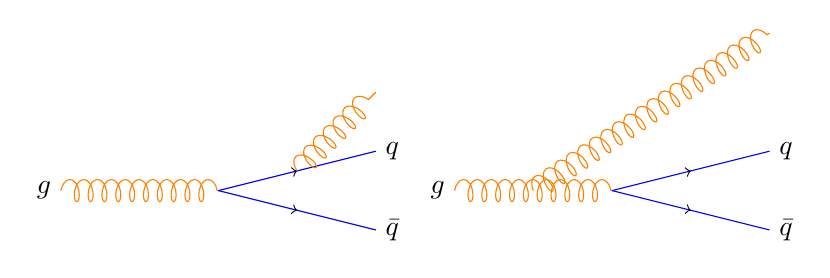
\begin{tikzpicture}[scale = 2]
\tikzset{
photon/.style={decorate, decoration={snake}, draw=red},
particlearrow/.style={draw=blue, postaction={decorate},
    decoration={markings,mark=at position .5 with {\arrow[draw=black]{>}}}},
antiparticlearrow/.style={draw=blue, postaction={decorate},
    decoration={markings,mark=at position .5 with {\arrow[draw=black]{>}}}},
particle/.style={draw=blue},
antiparticle/.style={draw=blue},
gluon/.style={decorate, draw=orange,
    decoration={coil,amplitude=4pt, segment length=5pt}}
 }
\coordinate[label=left:$g$] (a);
\coordinate[right=2cm of a] (vertex);
\coordinate[above right = 0.25cm and 1cm of vertex] (vertex2);
\coordinate[above right=1cm and 1cm of vertex2] (gluon);
\coordinate[above right=0.5cm and 2 cm of vertex,label=right:$q$] (b);
\coordinate[below right=0.5cm and 2 cm of vertex,label=right:$\bar q$] (c);
\draw[gluon] (a) -- (vertex);
\draw[particlearrow] (vertex) --  (b);
\draw[particlearrow] (vertex) --  (c);
\draw[gluon] (vertex2) -- (gluon);

\coordinate[label=left:$g$,right=3cm of vertex] (g2);
\coordinate[right=2cm of g2] (vertex3);
\coordinate[left = 1cm of vertex3] (vertex4);
\coordinate[above right=2cm and 3cm of vertex4] (gluon2);
\coordinate[above right=0.5cm and 2 cm of vertex3,label=right:$q$] (b2);
\coordinate[below right=0.5cm and 2 cm of vertex3,label=right:$\bar q$] (c2);
\draw[gluon] (g2) -- (vertex3);
\draw[particlearrow] (vertex3) --  (b2);
\draw[particlearrow] (vertex3) --  (c2);
\draw[gluon] (vertex4) -- (gluon2);
\end{tikzpicture}

\caption{Soft gluon production}
\label{fig:soft}
\end{figure}
When a gluon splits into two quarks one of the produced quarks can emit a soft gluon as seen in Figure~\ref{fig:soft}. In the laboratory frame the time it takes for a gluon to be emitted from a quark can be estimated to be~\cite{basicsofpqcd}
\nobreak


\begin{equation}
t_\mathrm{emit} \approx \frac{1}{E_q},
\end{equation}
\nobreak
\noindent where the energy of the quark is given by $E_q$. In the rest frame of the quark its energy is set by its virtuality $M_\mathrm{virt}$. With the assumption that the quark is massless the Lorentz factor from the rest frame to the laboratory frame is 

\begin{equation}
\gamma = \frac{E_q}{M_\mathrm{virt}}.
\end{equation}

\noindent Thus the emission time can be written as

\begin{equation}
t_\mathrm{emit} \approx \frac{E_q}{M_\mathrm{virt}^2}  = \frac{E_q}{\left(k+p\right)^2},
\end{equation}
\noindent where $k$ and $p$ are the four-momenta of the gluon and the quark after the gluon emission. As the square of a four-momentum is Lorentz invariant, this can be expanded in the laboratory frame. Assuming that the end products are massless, this leads to a form where the gluon emission time is expressed by the opening angle $\theta_\mathrm{kq}$ between the quark and the gluon


\begin{equation}
t_\mathrm{emit} \approx \frac{1}{k\theta_\mathrm{kq}^2}.
\end{equation}


\noindent The transverse wavelength of the emitted gluon is $\lambda_\perp^{-1}=k_\perp\approx k\theta_\mathrm{kq}$. This gives

\begin{equation}
t_\mathrm{emit} \approx \frac{\lambda_\perp}{\theta_\mathrm{kq}}.
\end{equation}

\noindent The secondary gluon can only probe the quark of the earlier splitting if the transverse wavelength is smaller than the transverse separation of the produced $\mathrm{q \bar q}$ pair, which is given by

\begin{equation}
r_\perp^{\mathrm{q \bar q}} \approx \theta_\mathrm{q \bar q} t_\mathrm{emit} \approx \lambda_\perp \frac{\theta_\mathrm{q \bar q} }{\theta_\mathrm{k q} }.
\end{equation}

\noindent Thus in order for the emission to probe the individual quark, the opening angle of the $\mathrm{q \bar q}$ splitting, $\theta_\mathrm{q \bar q}$, must be larger than $\theta_\mathrm{k q}$. If the opening angle $\theta_\mathrm{k q}$ is larger, the gluon can't distinguish between the quark and the antiquark, and it can only probe the state of the system before the splitting. Thus it is indistinguishable from a gluon emitted by the primary gluon.

This leads to the angular ordering of soft gluon radiation. Each successive radiated gluon must be at a smaller angle than the previous one. The effect can be calculated in all orders ~\cite{basicsofpqcd} and in the DGLAP formalism one can select the evolution variable $Q^2$ in a way that ensures angular ordering as is done in the Herwig MC generator~\cite{herwigManual}. In \pythia~8 this is strictly not included, but the transverse momentum ordered showers can describe the soft gluon emissions with similar accuracy as the angular ordered showers~\cite{eventGenerators}.




\subsubsection{Jet hadronisation}
When the virtuality of the shower is low enough, the shower starts to hadronise. In this regime the parton shower reaches an energy scale close to $\Lambda_{\mathrm{QCD}}$ and the perturbative description is no longer valid. Thus the hadronisation stage must be described in a non-perturbative manner. In general hadronisation is assumed to be universal, i.e. it should be independent of the collision energy and the collision system. 
The simplest model that is used in several theory approaches is the local parton-hadron duality hypothesis~\cite{Azimov1985}. In this hypothesis it is assumed that there exists a low virtuality scale $Q_0$ in which the hadronisation happens, that does not depend on the scale of the primary hard process. At this scale the partons transform into hadrons and their quantum numbers and flow of momentum directly gives those of the hadrons, with only small normalising corrections.

The next sections will present more complicated hadronisation models used in Monte Carlo generators, \pythia~and Herwig.

\subsubsection*{Lund string model}

One common implementation in MC generators is the Lund string fragmentation algorithm~\cite{ANDERSSON198331}. This is also used in the \pythia~generator. The string model utilises the fact that in QCD linear confinement is expected over large distances~\cite{eventGenerators}. This can be modelled by imagining a colour flux tube being extended between outgoing partons as illustrated in Figure ~\ref{fig:fluxtube}(a) for a $\mathrm{q \bar q}$-pair. The tube is assumed to have a uniform fixed transverse size of about \unit[1]{fm} along its length, which leads to a linearly rising potential $V\left(r\right) = \kappa r$, where the string constant $\kappa$ describes the amount of energy per unit length. A value of $\kappa \approx \unit[1]{\GeVfm} \approx\unit[0.2]{GeV^2}$ can be obtained from hadron mass spectroscopy~\cite{eventGenerators}.

The evolution of string fragmentation is illustrated schematically in Figure~\ref{fig:fluxtube}(b). The evolution is shown in a light cone presentation, i.e. the initial quark and antiquark are moving in opposite directions at the speed of light. The horizontal red line illustrates the string between the quark-antiquark pair. The string begins to stretch which continues until the potential energy stored in the string is large enough and it breaks, which forms a new quark-antiquark pair. If the original pair was $\mathrm{q \bar q}$ and the produced pair is $\mathrm{q'\bar q'}$, these form new pairs, $\mathrm{q \bar q'}$ and $\mathrm{q'\bar q}$.

Since these produced pairs are also moving away from each other, the strings between them will also stretch and can eventually break, creating even more pairs. This evolution proceeds until the invariant mass of the system becomes small enough and a group of final state mesons is formed. 

\begin{figure}
\centering
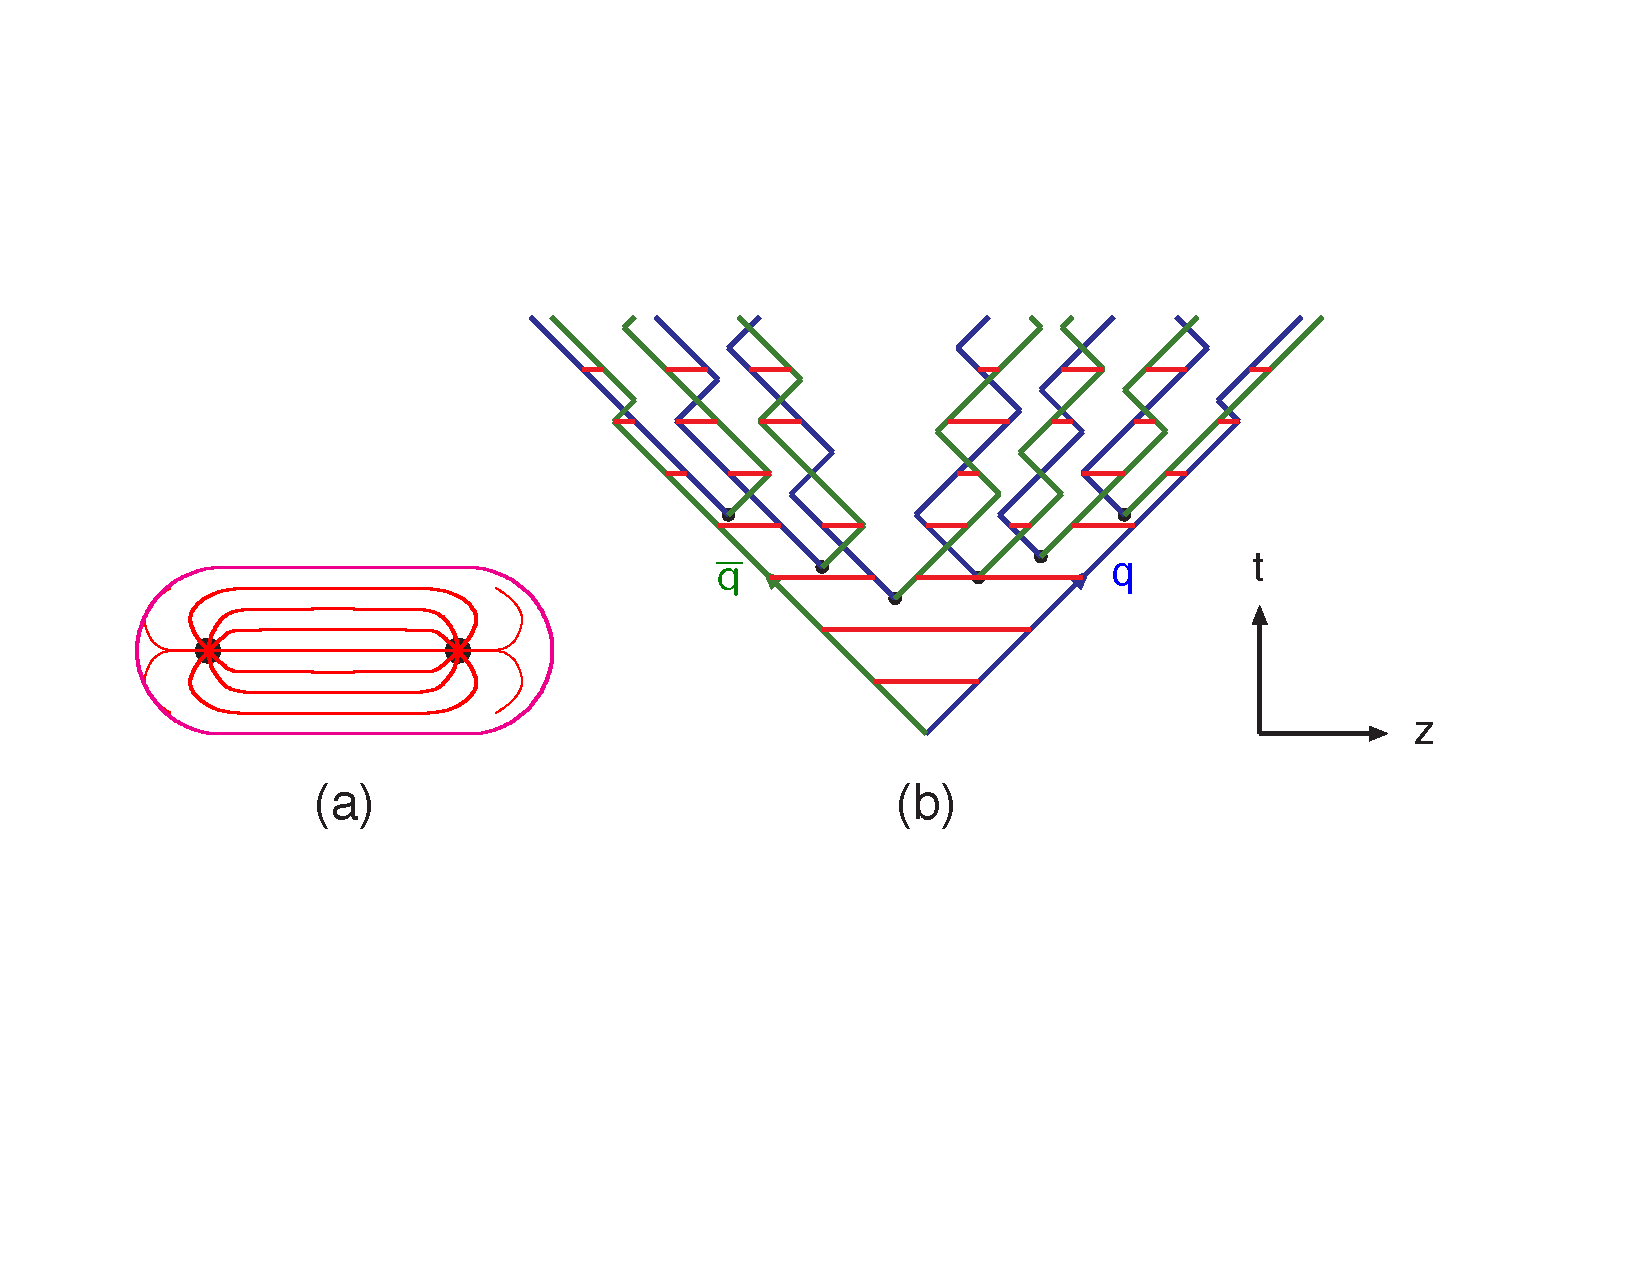
\includegraphics[width=0.75\textwidth]{pics/stringone.pdf}
\caption[]{ (a) A flux tube spanned between a quark and an antiquark. (b) The motion
and breakup of a string system, with the two transverse degrees of freedom suppressed
(diagonal lines are (anti)quarks, horizontal ones snapshots of the string field) \cite{eventGenerators}.
 }
\label{fig:fluxtube}
\end{figure}

To mathematically model the string the Lund model uses a massless relativistic string that has no transverse degrees of freedom.  When a string breaks the pair is created at one point and the pair then tunnels out to a classically allowed region. Therefore the probability to create a new quark-antiquark pair is proportional to the tunnelling probability~\cite{ANDERSSON198331}


\begin{equation}
P_\mathrm{tunnelling} \propto \exp \left(\frac{-\pi m_\mathrm{T}^2}{\kappa} \right) = \exp \left(\frac{-\pi m^2}{\kappa} \right) \left(\frac{-\pi \pt{}^2}{\kappa} \right),
\end{equation}

\noindent where the transverse mass $m_\mathrm{T}$ is defined as $m_\mathrm{T}^2 = m^2 + \pt{} ^2$. Here transverse refers to the plane transverse to the string axis. This equation gives a flavour-independent Gaussian $\pt{}$-distribution for the created $\mathrm{q \bar q}$ pairs.

In this formalism the string fragmentation would only produce mesons, but we know that also baryons are created in the process. To produce baryons the model introduces a probability for the creation of a diquark-antidiquark pair instead of a quark-antiquark pair when a string breaks. 

An iterative procedure is used to determine the kinematics of string breakages. The string fragmentation can be considered in any order, as there is no natural ordering. One can start from the quark leg and work one's way to the $\bar{\mathrm{q}}$ leg, or vice versa. This will give a left-right symmetry to the string fragmentation. To break the string into a hadron and the remaining system, the Lund model defines a symmetric fragmentation function as

\begin{equation}
f\left(z\right) \propto \frac{1}{z} \left(1-z\right)^a \exp \left(-\frac{b m_\mathrm{T} ^2}{z} \right),
\label{eq:symmetric}
\end{equation}

\noindent where $z$ is the fraction of light-cone momentum $p^+$ that the hadron obtains in the string breakage, $m_\mathrm{T}$ is the transverse mass of the hadron and $a$ and $b$ are tuneable model parameters. For heavy quarks this is modified as 

\begin{equation}
f\left(z\right) \propto \frac{1}{z^{1+bm_Q^2}} \left(1-z\right)^a \exp \left(-\frac{b m_\perp ^2}{z} \right).
\label{eq:symmetric2}
\end{equation}

\noindent Thus the process starts from the quark leg of a $\mathrm{q \bar{q}}$ system and then considers the breaking into a new $\mathrm{q' \bar q'}$ pair closest to the q-leg. After this breakage there is a meson $\mathrm{q \bar{q}'}$ and a remainder system spanning from $\mathrm{q' \bar{q}}$. This process continues until the antiquark leg is reached. Small corrections are required for the final two hadrons coming from a string as Equation (\ref{eq:symmetric}) assumes that the mass of the remainder system is large.
%A small detail here is that in equation (\ref{eq:symmetric}) it is assumed that the mass of the remainder system is large. Thus some patching up is needed for the last two hadrons coming from a string. The patching up is done such that the place where it happens looks as closely like any other string break as possible.

One additional possibility one must consider is that a string can have such a low mass that it cannot break at all. For these cases the string is transformed into a single hadron and if necessary energy and momentum are exchanged with other partons in the event.

Some of the produced hadrons are short-lived ones which can still decay. The final set of particles is obtained when these have decayed~\cite{introPythia82}.


\subsubsection*{Cluster model}
Instead of a string model HERWIG~\cite{herwigManual} uses a cluster model for hadronisation. The advantage of cluster models is that they require a smaller number of parameters than string models. The model is based on the preconfinement property of parton showers, i.e. the colour structure of a shower at any evolution scale $Q_0$ is such that colour singlet combinations of partons can be formed with an asymptotically universal invariant mass distribution. The invariant mass is independent of the initial hard process scale $Q$, and depends only on $Q_0$ and the QCD scale $\Lambda _ \mathrm{QCD}$, when $Q \gg Q_0$~\cite{eventGenerators}.

The cluster model starts by transforming all gluons non-perturbatively into $\mathrm{q \bar q}$ pairs, which requires that the gluons get a mass at least twice the lightest quark mass. When the gluons have been transformed into quarks, adjacent colour lines can clustered into colour singlets that have mesonic quantum numbers. The sum of the momenta of partons defines the momentum of the entire cluster. The principle of colour-preconfinement states that the mass distribution of these clusters is independent of the hard scattering process and its centre-of-mass energy~\cite{herwigManual}. %As the mass distribution is peaked at low masses, the clusters can be regarded as highly excited hadron resonances and decayed into the final state hadrons.

The mass of some of these initial clusters can be too large to reasonably describe an excited hadron and they must be split before they are allowed to decay. The condition to split cluster $C$ is~\cite{herwigManual}

\begin{equation}
M_C^p \geq M_\mathrm{max}^p  + \left( m_1 + m_2\right)^p,
\label{eq:clustermass}
\end{equation}

\noindent where $m_{1,2}$ are the masses of the constituents partons of the cluster. $M_\mathrm{max}$ and $p$ are parameters defined in the model. These have to be chosen separately for clusters containing light, charmed and bottom quarks. When a cluster splits, a pair of quarks is generated from the vacuum, which combined with the original quark-antiquark pair form two new clusters. This process continues until no clusters with masses fulfilling Equation ~\ref{eq:clustermass} remain.

\begin{figure}
\centering
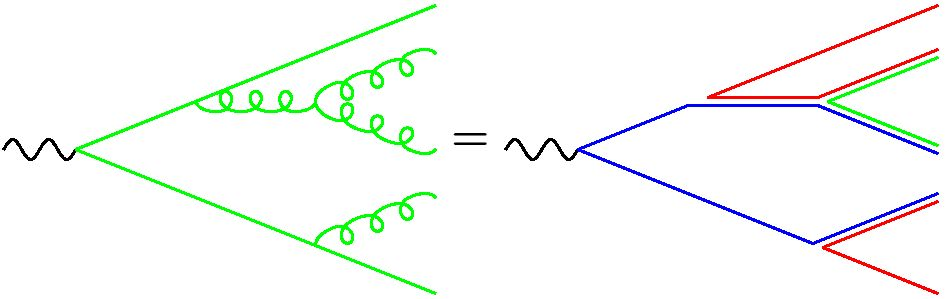
\includegraphics[width=0.75\textwidth]{pics/planar.jpg}
\caption[]{ Colour structure of a parton shower to leading order in $N_c$
\cite{eventGenerators} }
\label{fig:colourstructure}
\end{figure}

When all clusters are light enough, they decay into final state hadrons. If the cluster mass is high enough for decaying into a baryon-antibaryon pair, it can undergo either a mesonic or a baryonic decay. The probabilities of mesonic and baryonic decays are parameters in the model~\cite{herwigManual}. For a mesonic decay a quark-antiquark pair is created from the vacuum and for baryonic decays a diquark-antidiquark pair is made. Exact decay products get chosen by the model and cluster decays such that the decay is isotropic in the cluster rest frame. Any partons produced in the perturbative phase involved in the decay retain their original direction in the cluster rest frame. In cases where the cluster mass is too low to decay into a pair of mesons, some energy and momentum is exchanged with adjacent clusters so that it can decay into the lightest possible hadron. At the end the process gives a set of final state hadrons, some of which may be short-lived and decay before the end of the simulation~\cite{herwigManual}.

\subsubsection{Interactions between jet and medium}
Let us now look at what happens to jet production in heavy-ion collisions. Figure ~\ref{fig:jetq} shows a dijet produced inside QGP medium. High momentum particles are very rare and they are only produced in the initial collisions. In a heavy-ion collision, where a QGP medium is formed, the partons from a hard scattering are expected to interact strongly with the medium due to their colour charges and thus lose energy, either through gluon bremsstrahlung, or through collisions with medium partons~\cite{Connors:2017ptx}. This is referred to as jet quenching.  Studying the modification of jets inside the medium gives another key approach to constraining the properties of QGP. Modification can be also observed in jet shapes, particle composition, fragmentation, splitting functions and many others.


\begin{figure}
\centering
\documentclass{standalone}
\usepackage{tikz}
\usepackage{xcolor}
\usetikzlibrary{shapes,arrows}
\usetikzlibrary{trees}
\usetikzlibrary{shadows.blur}
\usetikzlibrary{positioning}
\usetikzlibrary{decorations.pathmorphing}
\usetikzlibrary{decorations.markings}
\begin{document}

\tikzset{
photon/.style={decorate, decoration={snake}, draw=red},
particlearrow/.style={draw=blue, postaction={decorate},
    decoration={markings,mark=at position .5 with {\arrow[draw=black]{>}}}},
antiparticlearrow/.style={draw=blue, postaction={decorate},
    decoration={markings,mark=at position .5 with {\arrow[draw=black]{>}}}},
particle/.style={draw=blue},
antiparticle/.style={draw=blue},
gluon/.style={decorate, draw=black,
    decoration={coil,amplitude=4pt, segment length=5pt}}
 }
 
 
 
\tikzstyle{proton} = [ellipse, draw=black, text centered, fill=orange!20, minimum height=3cm, blur shadow = {shadow blur steps=5},minimum width=1em ] 
\tikzstyle{protonnoshade} = [ellipse, draw=black, text centered, fill=orange!20, minimum height=3cmminimum width=1em ] 

\begin{tikzpicture}[node distance=1cm and 1.5cm]
\node[proton]  (proton)  {};
\node[proton, right=5cm of proton] (proton2) {};
\coordinate[above right=-0.5cm and 0.03cm of proton] (aux2);
\coordinate[below =0cm of proton] (a);
\coordinate[above=0cm of proton2] (b);
\shade[inner color=red, outer color=yellow] (a) rectangle (b);

\coordinate[right=-0.75cm and 2.5cm of aux2] (vertex1);
\coordinate[left=2cm of proton2] (vertex2);
\node[proton]  (proton3)  {};
\node[proton, right=5cm of proton] (proton4) {};

%\coordinate[below right=1.5cm and 0.5cm of vertex1] (vertex2);

%\coordinate[below right=0.0cm and 2cm of vertex2] (b1);
%\node[proton, below right=-0.05cm and 0.02cm of b1] (proton2) {};
%\coordinate[left=2cm of proton2] (aux6);
%\coordinate[below left=-0.05cm and 0.02cm of proton2] (b2);
%\coordinate[left=2cm of b2] (aux7);
%\coordinate[left=2cm of aux7] (spec3);
%\coordinate[left=2cm of aux6] (spec4);
%\coordinate[right of=proton2] (p2);
\coordinate[above right=1cm and 1cm of vertex1] (jet1);
\coordinate[below left=1cm and 1cm of vertex2] (jet2);


%Jet cones
\coordinate[above right=1cm and 0.5cm of jet1] (cone11);
\coordinate[above right=0.5cm and 1cm of jet1, label={right:Jet}] (cone12);
\draw[particle] (jet1) -- (cone11);
\draw[particle] (jet1) -- (cone12);
\draw[blue] (cone11) to[out=45,in=45]  (cone12);
\draw[blue] (cone11) to[out=225,in=225] (cone12);

\coordinate[below left=1cm and 0.5cm of jet2] (cone21);
\coordinate[below left=0.5cm and 1cm of jet2, label={left:Jet}] (cone22);
\draw[particle] (jet2) -- (cone21);
\draw[particle] (jet2) -- (cone22);
\draw[blue] (cone21) to[out=45,in=45]  (cone22);
\draw[blue] (cone21) to[out=225,in=225] (cone22);

\draw[particlearrow] (aux2) -- node[label=below:$q$] {} (vertex1); 
\draw[particle] (vertex1) -- (jet1);
\draw[particle] (vertex2) -- (jet2);

\draw[gluon] (vertex1) -- (vertex2);
\draw[particlearrow] (proton2) -- node[label=above:$q$] {} (vertex2);

%\draw[particlearrow] (p2) -- node[label=above:$P_B$] {} (proton2);




\end{tikzpicture}



\end{document}

\caption{If hard scatterings happen in conjunction with QGP medium the produced jets must traverse the medium. Thus they are subject to interactions with the medium. Note that the dijet pair can be created anywhere within the medium volume and thus the two jets will have differing path lengths through the medium.}
\label{fig:jetq}
\end{figure}

\subsubsection*{Discovery of jet quenching via leading hadron suppression}
\label{sec:energyloss}
First evidence of jet quenching comes from observing high $\pt{}$ tracks, i.e. the leading hadrons of jets. In this picture jet energy loss in heavy-ion collisions is usually quantified with the nuclear modification factor $R_{AA}$, which is  is defined as
%the yield in heavy-ion collisions divided by the yield in proton-proton collisions and scaled by the The nuclear modification factor

\begin{equation}
R_{AA}\left(\pt{}\right) = \frac{(1/N_{AA}^{evt})\dd {N^{AA}}/\dd {\pt{}}}{\left< N_{coll}\right> (1/N_{pp}^{evt})\dd {N^{pp}}/\dd {\pt{}}}\label{eq:raa}
\end{equation}
\noindent where $\dd{N^{AA}}/\dd{\pt{}}$ and $\dd{N^{pp}}/\dd{\pt{}}$ are the observed spectra in heavy-ion and proton-proton collisions, respectively and $\left< N_{coll}\right>$ is the average number of binary nucleon-nucleon collisions in one heavy-ion event, which can be calculated from the Glauber model as shown in Section~\ref{sec:geometry}. When studying direct production of high $\pt{}$ tracks a heavy-ion collision can be estimated relatively well to be only a combination of individual proton-proton collisions. At low $\pt{}$ this scaling breaks down as the determining factor in direct production is the number of participants.


\begin{figure}[hbt]
	\centering
                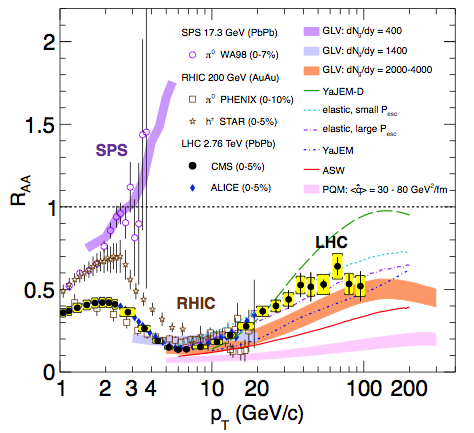
\includegraphics[width=0.65\textwidth]{pics/Raaplot}
        \caption[Measurements of the nuclear modification factor $R_{AA}$ in central heavy-ion collisions]{Measurements of the nuclear modification factor $R_{AA}$ as a function of \pt{} in central heavy-ion collisions at three different centre-of-mass energies. Separate results are shown for different particle species~\cite{Aamodt:2010jd, Aggarwal:2001gn, d'Enterria:2004ig, Adare:2008qa, Adams:2003kv,CMS:2012aa} and the results are compared to predictions from several theoretical calculations~\cite{Dainese:2004te, Vitev:2002pf, Vitev:2004bh, Salgado:2003gb, Armesto:2005iq, Renk:2011gj}.}
        \label{fig:Raa}
\end{figure}

If the medium has no effect on high $\pt{}$ particles the nuclear modification factor should be 1. As seen in Figure~\ref{fig:Raa} $R_{AA}$ at RHIC and LHC has been observed to be as low as 0.2, which is a clear signal that jet quenching is happening. However, the physical interpretation is not that 80 \% of high momentum tracks disappear, rather they are shifted to smaller momenta. The relation between the shift in momentum and $R_{AA}$ depends on the steepness of the $\dd{N}/\dd{\pt{}}$ spectra. At LHC energies the spectrum is flatter and thus the same $R_{AA}$ value as in RHIC requires a larger momentum shift, which results from the larger temperature of the medium at LHC. 

The reaction plane dependence of inclusive particle $R_{AA}$ demonstrates that energy loss is path length dependent~\cite{Adler:2006bw}, as expected from models. The path length can be affected by collisions centrality and system size. However, the temperature and lifetime of the QGP also changes with changing centrality and system size. Thus to study different path lengths the angle relative to the reaction plane gives the cleanest signal, as the properties of medium remain the same. Additionally it was concluded that there is no suppression for path lengths below $\mathrm{L} = \unit[2]{fm}$. Similar indications about path length dependence are given by jet $v_2$ both at RHIC~\cite{Adare:2013wop} and at LHC~\cite{Abelev:2012di,Chatrchyan:2012xq}. 



 %Naturally jet quenching depends on the path lengths through the medium.

%\subsubsection*{Theory of jet quenching}


%After the hard partons are created they escape the medium before a thermal equilibrium is reached. Thus they are not part of the pressure-driven collective expansion. Instead high momentum yield is suppressed because of energy loss in the medium. When propagating through the medium these partons lose energy as they pass through the medium. This is referred to as jet quenching. Jet quenching depends on the path lengths through the medium. Thus anisotropy in this region is mainly dependent on the collision geometry and density of medium.


%The energy loss of partons in medium is mainly due to QCD bremsstrahlung and to elastic scatterings between the parton and the medium. 


\subsubsection*{QED Bremsstrahlung}
In modelling energy loss in QCD medium it is often useful to consider the analogy to the QED process, where an electron propagating through matter loses energy through photon Bremsstrahlung radiation. In the simplest case, each individual scattering centre results in a single emission of a photon. This is known as the Bethe-Heitler regime~\cite{BetheHeitler}. In this regime the energy spectrum of radiated photons $\nicefrac{\dd N}{\dd E}$ is proportional to $\nicefrac{1}{E}$. However this radiation requires that the distance between scattering centres is larger than the formation length of the photon. When the scattering centres are closer than the formation length, the radiation process becomes suppressed. This phenomenon is known as the Landau-Pomeranchuk-Migdal (LPM)~\cite{Landau:1953um,Migdal:1956tc} suppression. In this energy regime the radiated spectrum is proportional to $\nicefrac{1}{\sqrt{E}}$.

Further suppression to low energy photons comes from the destructive interference leading to the suppression of Bremsstrahlung photons of $E < \gamma \omega_p$, where $\omega_p$ is the plasma frequency of the radiator. This is knows as Dielectric suppression. The photon energy distribution in this regime is proportional to the energy of the photon. A schematic view of the effect of these three regimes is shown in Figure~\ref{fig:bremsstrahlung}.

\begin{figure}[htb]
\centering
\includegraphics[height=2in]{pics/BremsstrahlungElectron}
\caption[Photon spectrum]{ The expected bremsstrahlung spectrum for a electron propagating through material  ~\cite{Bosted1993QuantummechanicalSO} }
\label{fig:bremsstrahlung}
\end{figure}

\subsubsection*{QCD}
In QCD the radiative energy loss mechanism is given in terms of the transport coefficient $\left<\hat q\right>$, which describes the average momentum transfer between the medium and parton~\cite{jetBroadeningPpb1}. The exact definition of this depends on the theoretical formalism used to describe the energy loss mechanism. 

Similar to QED the simplest energy loss process is elastic QCD scattering off medium partons. In elastic scatterings a part of the energy of the scattered partons is absorbed by the thermal QGP medium and the energy of the initial parton is reduced. The mean energy loss caused by elastic scatterings can be estimated by

\begin{equation}
\left<\Delta E\right>_{\mathrm{el}}=\sigma \rho L \left<E\right>_{\mathrm{1\,scatt}}\propto L,
\label{eq:elastic}
\end{equation}

\noindent where $\sigma$ is the interaction cross section and $\left<E\right>_{1 scatt}$ is the mean energy transfer of one individual scattering~\cite{Majumder:2010qh}. This requires that the energy transfer does not depend on the total energy of the parton ($E$). The mean energy loss per path length is defined to be the transport coefficient \begin{equation}
\left< \hat q_\mathrm{el}\right> = \nicefrac{\left< \Delta E\right>}{L}.
\end{equation}

An alternative energy loss mechanism is medium-induced radiation. In QCD this radiation is mainly due to the elementary splitting processes, $q\rightarrow qg_r$ and $g\rightarrow gg_r$. In the limit where the parton is moving with the speed of light radiation energy loss is given by

\begin{equation}
\left<\Delta E\right>_{rad}\propto T^3L^2,
\label{eq:radiative}
\end{equation}

\noindent where $L$ is the path length through the medium and $T$ is the medium temperature~\cite{Dominguez:2008vd}. The different exponents of $L$ in equations \ref{eq:elastic} and \ref{eq:radiative} indicate that radiative energy loss is dominant over elastic energy loss.

Several models have been used to attempt describing the mechanism of energy loss. The most used formalisms can be divided into four approaches.
%
%\begin{itemize}
%\item Thermal effective theory formulation (AMY)~\cite{Arnold:2001ms, Arnold:2002ja}
%\item Opacity Expansion ((D)GLV/WHDG and ASW-SH)~\cite{Salgado:2003gb, Gyulassy:2000er, Gyulassy:1999zd, Wiedemann:2000za} 
%\item Higher Twist approach~\cite{Wang:2001ifa, Majumder:2009zu} 
%\item Multiple soft scattering approximation BDMPS-Z (ASW-MS)~\cite{Baier:1996kr, Zakharov:1996fv, Baier:1998kq, Salgado:2003gb}
%\end{itemize}

In the Gyulassy-Levai-Vitev (GLV)~\cite{Gyulassy:1999zd} opacity expansion model the radiative energy loss is considered at a few scattering centres. Radiated gluons are constructed by pQCD calculations which sum up the relevant scattering amplitudes in terms of the number of scatterings. Another model using this opacity expansion approach is the ASW model by Armesto, Salgado and Wiedermann~\cite{Wiedemann:2000za}.

The second approach is the thermal effective theory formulation by Arnold, Moore and Yaffe (AMY)~\cite{Arnold:2001ms} uses dynamical scattering centres. The model uses leading order pQCD hard thermal loop effective field theory. In this model it is assumed that because of the high temperature of the QGP medium the coupling constant of the strong interaction can be treated as small. Partons, that propagate through the plasma, lose energy from both soft and hard scatterings.

These pQCD models consider the energy loss for a parton propagating through the medium. An alternative approach is the higher twist (HT) model by Wang and Guo~\cite{Wang:2001ifa} which considers the effect of energy loss on the energy scale evolution of fragmentation functions.

The fourth category includes the Monte Carlo methods. The \pythia~event generator~\cite{pythia} is widely used in high-energy particle physics. Although primarily used for proton-proton collisions, \pythia~was recently extended by the Angantyr~\cite{Bierlich:2018xfw} model which implements some features of heavy-ion collisions. Other Monte Carlo models based on \pythia~describing the energy loss mechanism are PYQUEN~\cite{Lokhtin:2005px} and Q-Pythia~\cite{Armesto:2009zc}. Other Monte Carlo models include JEWEL~\cite{Zapp:2008gi} and YaJEM~\cite{Renk:2009nz}. 





\subsubsection{New paradigm of jet Quenching}
As described in the previous sections the first indications of jet quenching, such as $R_{\mathrm{AA}}$, looked essentially at the leading hadrons of jets, the hard part, ignoring the soft scale part of jet phenomena. However, experimental methods have since improved; jet reconstruction algorithms have become reliable in the LHC era. Instead of the leading hadron we can study the entire jet shower and its structure. In jet observables one must consider what happens to the lost energy. Radiated gluons may end up being clustered with the jet, depending on the radiation angle, the parameters of jet reconstruction and whether the gluon reaches equilibrium with the medium or not. Thus the suppression on the jet level is expected to be smaller. Figure~\ref{fig:jetraa} shows jet $R_{AA}$ in central \PbPb collisions measured by ALICE, ATLAS and CMS and indeed jet $R_{AA}$ is about 0.5 instead of 0.2. %This raises the conceptual question, what counts as being part of the jet.  If a gluon radiated from the jet thermalises with the medium, is it a part of the jet or the medium?


%The first evidence of jet quenching in reconstructed jets at the LHC was observed by measuring the dijet asymmetry, $A_j$ ~\cite{Connors:2017ptx}.  


\begin{figure}
\centering
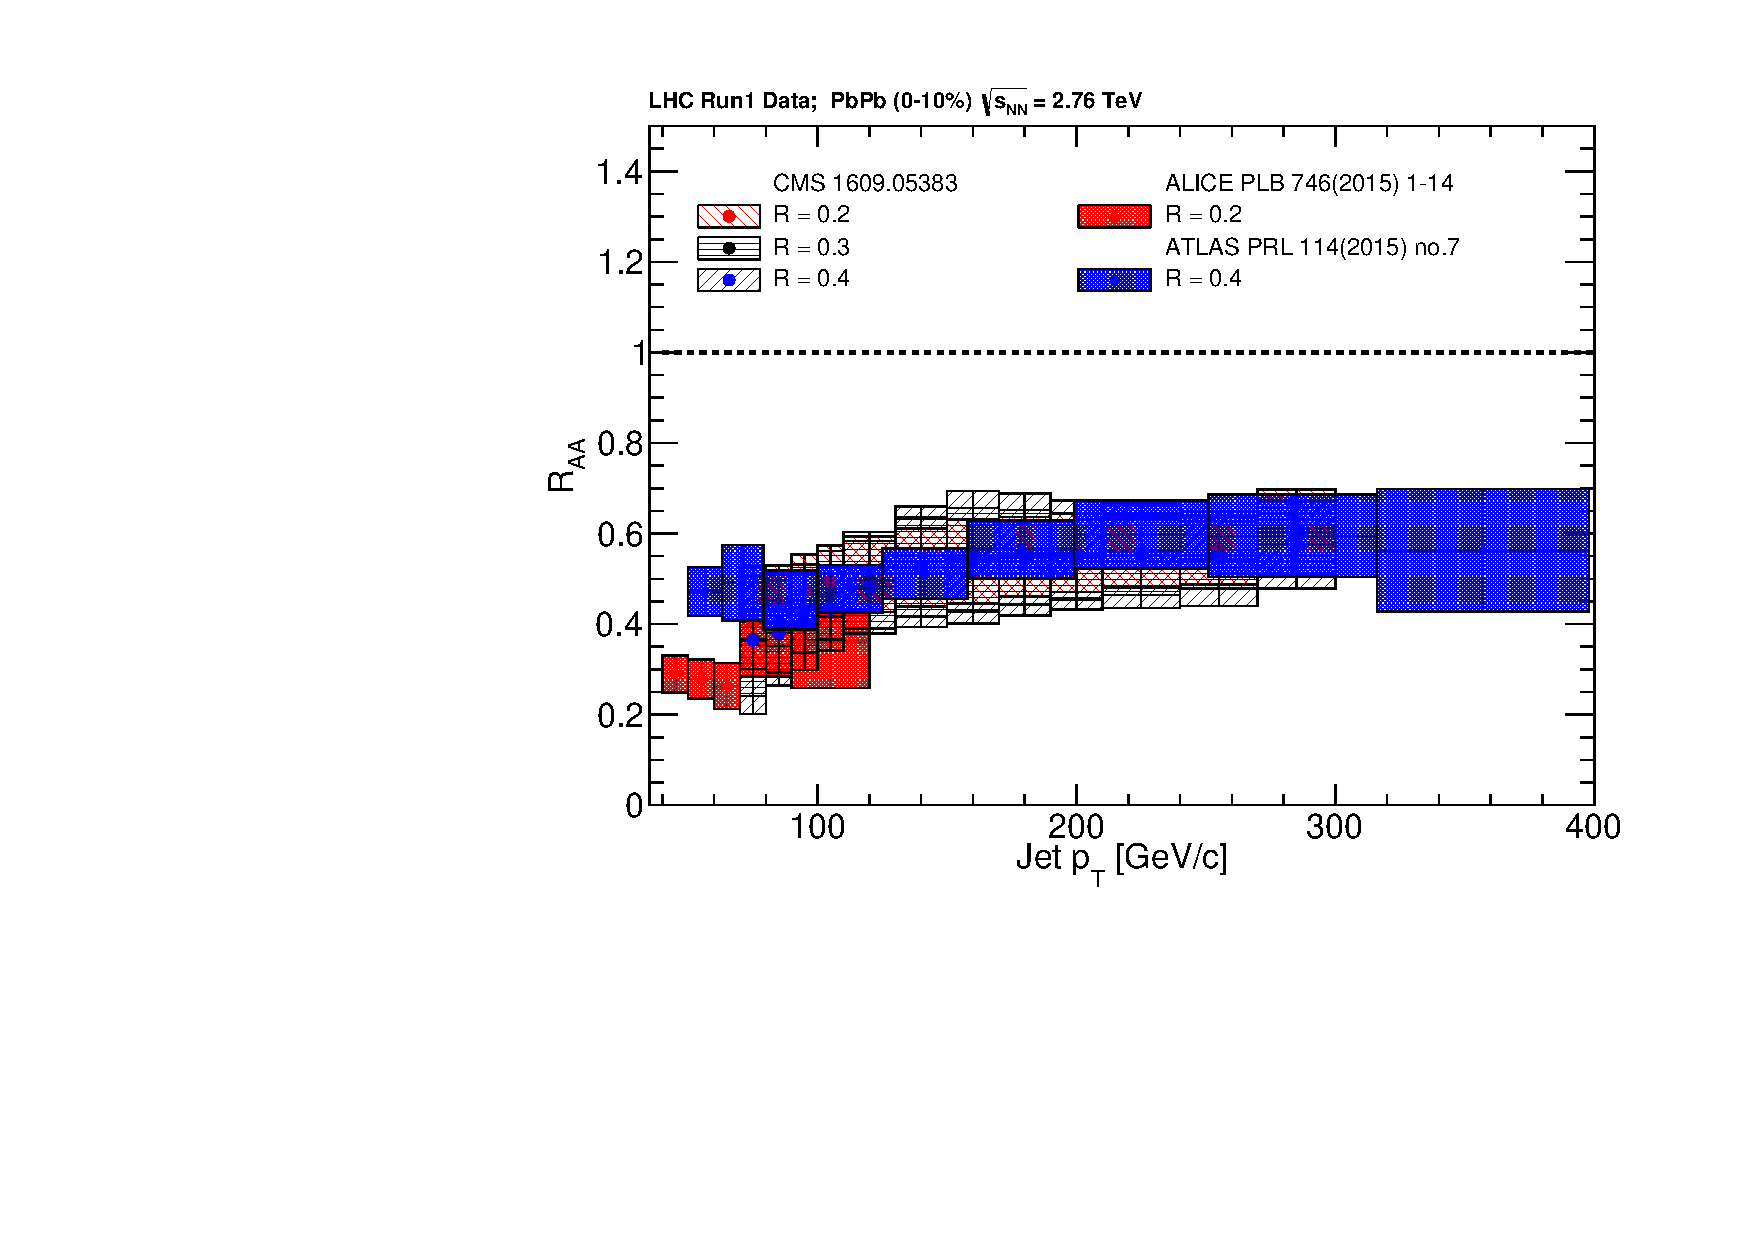
\includegraphics[height=2.4in]{figures/LHC_Run1_RAA_comparison_cent010.pdf}
 \caption{Reconstructed anti-$\kt{}$ jet $R_{AA}$ from ALICE~\cite{Adam:2015ewa} with $R = 0.2$ for $\left| \eta \right| < 0.5$, ATLAS~\cite{Aad:2014bxa} with $R = 0.4$ for $\left| \eta \right| < 2.1$, and CMS~\cite{Khachatryan:2016jfl} with R = 0.2, 0.3 and 0.4 for $ \left| \eta \right| < 2.0$. The ALICE and CMS data are consistent within uncertainties while the ATLAS data are higher. The experiments use slightly different methods in selecting jets and subtracting the underlying event contribution. Compared to ALICE and CMS the ATLAS technique could impose a survivor bias and lead to a higher jet $R_\mathrm{AA}$ at low momenta as argued in~\cite{Connors:2017ptx}.}
\label{fig:jetraa}
\end{figure}

Thus, on the level of the reconstructed jet, energy loss manifests itself as broadening and softening of the jet. This is seen for example in jet-hadron correlations. Figure~\ref{fig:jethadron} shows $\Delta \eta$ correlations with the leading jet. $\Delta \phi$ correlations have similar trends. Jets in heavy-ion collisions have been observed to be broader, than in proton-proton collisions. The strongest effect happens for low momentum tracks. These observations are consistent with expectations from various energy loss models. Additionally it was observed that the broadening was stronger for subleading jets than for leading jets, which indicates a bias towards selecting less modified jets as the leading jet. Jet hadron correlations have also been studied at RHIC with similar conclusion~\cite{Adamczyk:2013jei}.


\begin{figure}
\centering
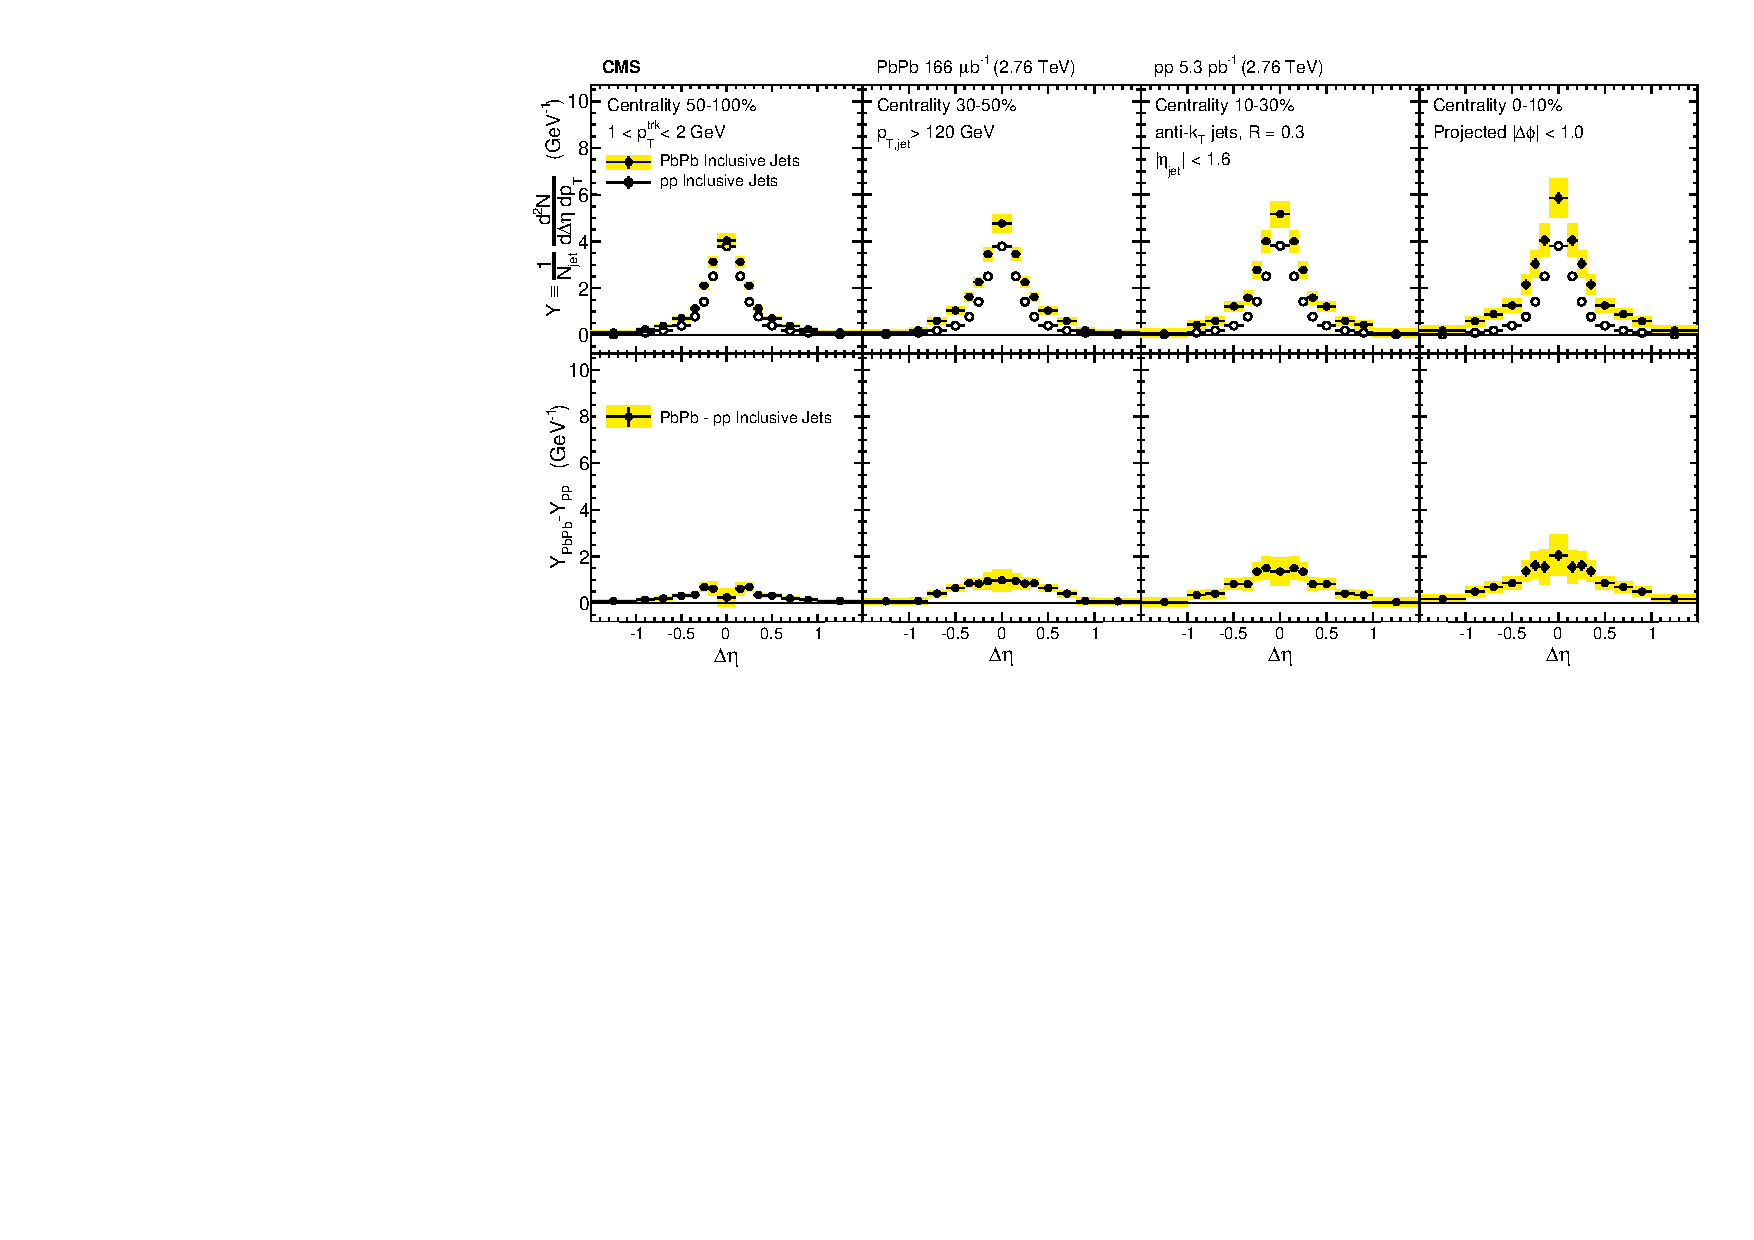
\includegraphics[height=2.4in]{figures/TrackJetCMS-HIN-14-016_Figure_003.pdf}
\caption{Measurement by CMS~\cite{Khachatryan:2016erx}. Symmetrized $\Delta \eta$ distributions correlated with \PbPb and \pp inclusive jets with $\pt{}>\unit[120]{\gev}$ are shown in the top panels for tracks with $1 < \pt{} < \unit[2]{\gev}$. The difference between per-jet yields in \PbPb and \pp collisions is shown in the bottom panels. These measurements indicate that the jet is broadened and softened, as expected. The effect is stronger in more central collisions.  $\Delta \phi$ correlations have similar trends.}
\label{fig:jethadron}
\end{figure}




\subsubsection*{Phase-space view of the medium modified parton cascade}
The new paradigm in jet quenching in heavy-ion collisions involves multi-scale problems~\cite{Kurkela:2014tla,Tachibana:2018yae}. The elementary scattering and the subsequent branching process down to non-perturbative scales are dominated by hard scales in the vacuum as well as in the medium. Soft scales, of the order of the temperature of the medium, characterise the interactions of soft partons produced in the shower with the QGP. Soft scales also rule hadronisation, which is expected to take place in vacuum for sufficiently energetic probes, even though some modifications can persist from modifications of colour flow~\cite{Aurenche:2011rd,Beraudo:2011bh,Beraudo:2012bq}. Understanding the contributions from the different processes to the jet shower evolution in medium and their scale dependence is crucial to to constrain the dynamics of jet energy loss in the expending medium, the role of colour coherence~\cite{CasalderreySolana:2012ef}, and fundamental medium properties like temperature dependent transport coefficient~\cite{DEramo:2012uzl,Ayala:2016pvm}.

\begin{figure}[tb]
\centering
\begin{subfigure}{0.48\textwidth}
\includegraphics[width=0.99\textwidth]{figures/regions4.eps}
%\caption[]{Illustration of how a medium-modified parton cascade fills the phase space. Early stage vacuum radiation dominates phase space in the DGLAP region. Late stage, after exiting the medium, radiation dominates the Late DGLAP regions.  }
%Parametrically accurate picture of how a medium-modified parton cascade fills the phase space. At time $t$, quanta can be formed up to momentum scale $k_{\rm form}$ and they are formed with $O(1)$ probability per $\log p$ at lower scale $k_{\rm split}$. Quanta below $k_{\rm split}$ split further and their energy cascades to the thermal scale $T$ in less than an epoch $t$. Transverse Brownian motion moves quanta up to the angle $\theta_{\rm BR}(p)$ denoted by the thick purple line.  The Moli\`ere region at larger $\theta$ is dominated by rare large angle scattering. At even larger angle, there are $O(\alpha_s)$ quanta per double logarithmic phase space  from DGLAP 'vacuum' radiation, and for momenta below $k_{\rm split}$ these cascade within time $t$ to $T$. After the jet escapes the medium, the jet and the emitted fragments will undergo vacuum radiation. This late time vacuum radiation emitted by the original parton dominates at sufficiently small $\log \theta$  (regions marked ``late DGLAP'' and bounded by $\theta_{\rm vac}$ and $\theta_\alpha$),  whereas the late time radiation of the fragments dominates in the region  denoted by ``Vacuum cascade of the medium induced quanta''. }
%\label{fig:cascades}
\end{subfigure}
\begin{subfigure}{0.48\textwidth}
\includegraphics[width=0.99\textwidth]{figures/e-vs-th3.eps}
%\caption[]{The distribution of energy as a function of angle for a fixed $p > k_\mathrm{split}$. The  Medium induced radiation dominates around the angular scale $\theta_\mathrm{BR}$. The medium induced contributions (dashed lines) grow as a function of evolution time with respect to the vacuum one (dotted line). ~\cite{Kurkela:2014tla}.}
%\label{fig:edistribution}
\end{subfigure}
\caption{{\it Left}: Phase space view of dominant contributions in a medium-modified parton cascade. {\it Right} The distribution of energy as a function of angle for a fixed momentum with $p > k_\mathrm{split}$. Large angular scales $\theta > \theta_\mathrm{Mol}$ are dominated by DGLAP vacuum radiation from the leading parton at the scale $Q$. At $\theta < \theta_\alpha$ the energy density is dominated by vacuum radiation of the leading parton after it has degraded its energy propagating through the medium. Areas $\theta_\alpha < \theta < \theta_\mathrm{BR}$ and $\theta_\mathrm{BR} < \theta < \theta_\mathrm{Mol}$ are dominated by Brownian motion and rare large angle (Moli\`ere) scatterings with medium partons ~\cite{Kurkela:2014tla}.}
\label{fig:cascades}
\end{figure}

Let us now look at medium modification of jets in a $\log\left(p\right)-\log\left(\theta\right)$ plane as shown in ~\cite{Kurkela:2014tla}. The different momentum and angular scales are subject to different physical phenomena. Figure~\ref{fig:cascades} shows the relevant medium modification phenomena for different regions of the phase space at time $t$, when a jet propagates through a thermal cloud of temperature $T$. As in a practice jets propagate over a finite path-length $L$ in QCD matter, Figure~\ref{fig:cascades} can be taken as a representation of the distribution of partonic jet fragments at moment $t \approx L$, when the jet escapes the medium~\cite{Kurkela:2014tla}.

The region marked as DGLAP is dominated by the primary vacuum splittings explained in section~\ref{sec:shower}. This region is determined by $\theta > \theta_\mathrm{vac}$ with

\begin{equation}
\theta_\mathrm{vac} \propto \nicefrac{1}{\sqrt{\pt{}}}.
\end{equation}


\noindent Medium-induced parton branching fills the $\log p$-$\log \theta$-plane from the bottom up (in $p$) and from the inside out (in $\theta$). This is because transverse momentum is acquired by Brownian motion in the medium, $k_\perp^2 \propto \hat q t$. The formation time constraint $t \geq \nicefrac{p}{k_\perp^2} \approx \nicefrac{p}{\hat q t}$ implies that medium-induced quanta can be formed in the region $p \leq k_\mathrm{form}$ where

\begin{equation}
k_\mathrm{form}\left(t\right) = \hat q t^2.
\end{equation}

\noindent For these splittees to survive without further splittings they must have 
\begin{equation}
p \geq k_\mathrm{split} \approx \alpha_s^2 k_\mathrm{form}\left(t\right) \approx \alpha_s^2\hat q t^2.
\end{equation} 

\noindent Thus the region marked as LPM in Figure~\ref{fig:cascades} is filled by the primary medium-induced branchings. Fragments with $p \leq k_\mathrm{split}$ will have time to split further. An approximately equal splitting where both splittees get momentum $~\nicefrac{p}{2}$ from the parent will degrade energy the most. These splittees will undergo the next splitting in an even shorter time scale producing even softer fragments. Momenta can continue cascading all the way to the thermal scale $T$ of the medium within the same time scale within which the first splitting occurred. Thus filling the region marked as Medium cascade in Figure~\ref{fig:cascades}. Similarly splittees from vacuum radiation can cascade inside the medium when they have $p \leq k_\mathrm{split}$, filling the bottom right corner of the $\log p$-$\log \theta$-plane.

%
%%\begin{equation}
%%\frac{\mathrm d P_\mathrm{find}\left(t\right)}{\mathrm d \log p} \propto \alpha_s \nicefrac{t}{t_\mathrm{form}}\left(p\right) \propto \alpha_s \hat q ^{\nicefrac{1}{2}} p^{-\nicefrac{1}{2}} t
%%\end{equation} 
%
%\noindent Not all quanta will stay where they were created. Those modes that have time to lose a significant fraction of their energy will cascade to a significantly lower scale $p$. For LPM-type radiation, the splitting that degrades energy the most is the hardest splitting. 
%
%The $\log p $ distribution has the same $\frac{1}{\sqrt{p}}$ dependence as in the LPM region
%
%\begin{equation}
%\frac{\mathrm{d}n}{\mathrm{d}\log p} = \frac{1}{p}\frac{\mathrm{d}\epsilon}{\mathrm{d}\log p} \approx \alpha_s \frac{\sqrt{\hat q t}}{\sqrt{p}}
%\end{equation}
%
%\noindent Also the quanta originating from the DGLAP region will undergo medium interactions that will make the quanta radiate and split. The distribution of radiation is the same as from any other mode. Above a certain momentum scale $k_\mathrm{split}$ the distribution of originating daughters is 
%
%
%\begin{equation}
%\frac{\mathrm d P_\mathrm{find}}{\mathrm d \log p \mathrm{d} \log \theta} \approx \alpha_s \frac{t}{t_\mathrm{split}\left(p\right)},
%\end{equation} 
%
%%\noindent Note that the ratio $\nicefrac{t}{t_\mathrm{split}}$ is smaller than 1 for nodes above $k_\mathrm{split}$ and therefore the number of daughters is smaller than the number of vacuum splitted quanta. Below $k_\mathrm{split}$ the cascade is similar to the medium cascade and the number of quanta become
%%
%%\begin{equation}
%%\frac{\mathrm{d}n}{\mathrm{d}\log p \mathrm{d} \log \theta} \approx \alpha_s \frac{t}{t_\mathrm{split}\left(p\right)}, \text{ for } p < k_\mathrm{split}\left(p\right)
%%\end{equation}


The angular distribution of the medium-induced radiation is driven by two mechanisms; Multiple soft scatterings give rise to transverse Brownian motion, which determines the distribution at small angles. The typical angle reached in the LPM region is 

\begin{equation}
\theta_\mathrm{BR}\left(p\right) \approx \frac{\sqrt{\hat q t}}{p}, \text{ for } k_\mathrm{form} > p > k_\mathrm{split},
\end{equation}

\noindent while in the medium cascade region of the phase space this becomes

\begin{equation}
\theta_\mathrm{BR}\left(p\right) \approx \left(\frac{T}{p}\right)^{\frac{3}{4}}
\end{equation}

\noindent Large angular scales cannot be reached by Brownian motion, but can arise from rare large angle scatterings with partons in the medium, described first by Molière~\cite{Moliere:1947zza}. The result is that medium-induced radiation is predominantly located in the bands marked as Brownian motion, where $\theta_\alpha < \theta < \theta_\mathrm{BR}$, and Moli\`ere, where $\theta_\mathrm{BR} < \theta < \theta_\mathrm{Mol}$ in Figure~\ref{fig:cascades}. 

The hard parton will naturally continue radiating after it leaves the medium. As there is no longer kinematic limits set by the time scale, the vacuum radiation can extend to smaller angular scales in the phase space. The results is that the regions, where $\theta<\theta_\alpha$, marked as Late DGLAP in Figure~\ref{fig:cascades} will be dominated by the late time vacuum radiation. Naturally also the splittees from medium-induced radiation will undergo the late stage vacuum radiation phase, filling the triangular region with small $p$ and $\theta < \theta_\mathrm{\alpha}$.



\subsubsection*{Influence of jet on medium}
Energy loss of hard partons is well established by experimental observations. Naturally energy can't just disappear, but is transferred to daughter partons or the medium. For radiation that stays inside the jet cone energy loss manifests itself as softening and broadening. If a daughter parton loses energy and becomes equilibrated with the medium it may no longer be correlated with the parent parton. This energy would then be distributed at distances far from the jet cone. There is some evidence for out-of-cone radiation by CMS~\cite{Chatrchyan:2011sx}, but the interpretation is not clear. Other possible phenomena include the mach cone and Moliére scattering, but there is no experimental evidence for these. Evidence for all of these effects is difficult to find as the underlying event gives already a large and fluctuating background. Additionally its unclear how this energy would be different from the underlying event~\cite{Connors:2017ptx}.
